\pdfminorversion=7
\pdfsuppresswarningpagegroup=1
\documentclass[namedate,webpdf,modern,mediumone]{oup-authoring-template}

\usepackage{booktabs,float,tabularx,array,etoolbox}
\graphicspath{{figures/}}
\newcommand{\societylogo}{}
\makeatletter
\patchcmd{\ps@opening}{\color{black!20}\rule{45pt}{55pt}}{}{}{}
\patchcmd{\ps@opening}{\color{black!20}\rule{45pt}{55pt}}{}{}{}
\makeatother
\usepackage[tablesonly,nomarkers,nolists]{endfloat}
\usepackage[section]{placeins}
\usepackage{xurl}
\hypersetup{colorlinks=true,linkcolor=blue,citecolor=blue,urlcolor=blue,
  pdftitle={Scale-dependent contraction of spatial wet-bulb temperature contrasts in eastern China},
  pdfauthor={Jian Hou, Tan Meng, and Maozai Tian}}
\setlength{\parindent}{0pt}
\setlength{\parskip}{1pt plus 0.5pt}
\setlength{\emergencystretch}{2em}
\setlength{\textfloatsep}{10pt plus 2pt minus 2pt}
\setlength{\floatsep}{8pt plus 2pt minus 2pt}
\setlength{\intextsep}{10pt plus 2pt minus 2pt}
\renewcommand{\efloatseparator}{\vspace{5pt}}

% Show the supplied descriptions directly below the figure legends for submission.
\renewcommand{\figalttext}[2][]{\par\smallskip
  {\footnotesize\raggedright\noindent\textbf{Alt text: }#2\par}}

\newcommand{\Var}{\mathrm{Var}}
\newcolumntype{Y}{>{\raggedright\arraybackslash}X}

\raggedbottom
\begin{document}

\journaltitle{Journal of the Royal Statistical Society Series C: Applied Statistics}
\copyrightyear{}
\pubyear{}
\lastpage{19}
\title[Spatial wet-bulb contrast contraction]{Scale-dependent contraction of spatial wet-bulb temperature contrasts in eastern China}
\author[1]{Jian Hou\ORCID{0000-0002-9248-6874}}
\author[2]{Tan Meng\ORCID{0009-0001-1812-1834}}
\author[2,$\ast$]{Maozai Tian\ORCID{0000-0002-0515-4477}}
\address[1]{\orgdiv{College of Systems Engineering}, \orgname{National University of Defense Technology}, \orgaddress{Changsha 410073, \country{China}}}
\address[2]{\orgdiv{Center for Applied Statistics, School of Statistics}, \orgname{Renmin University of China}, \orgaddress{\street{59 Zhongguancun Street}, Beijing 100872, \country{China}}}
\corresp[$\ast$]{Corresponding author. \href{mailto:mztian@ruc.edu.cn}{mztian@ruc.edu.cn}}

\abstract{
We examine how the spatial organisation of humid heat changes when regional
wet-bulb temperature is high. Synchronous fields over eastern China are
compared within summer months across 33 evaluation summers. A multiscale
graph analysis expresses regional dispersion and its spatial components
within the same relative contrast. The mean squared pairwise contrast is
$7.28\%$ lower on high-mean days, with attenuation concentrated in the broad
latitudinal structure. Broad-scale anomaly energy changes little; the contraction
is associated with anomalies opposing the monthly climatological gradient.
On a nested observation grid, these days also exhibit a wider connected
humid-heat footprint. At $24^\circ$C, total and largest connected exceedance
fractions are each approximately 13 percentage points greater than on middle
days. The coverage difference varies across temperature thresholds.
Simple spatial summaries retain most coverage information, while the graph
profile identifies the scales and structures of the dispersion change.
Historical and station comparisons support the broad pattern. The results
distinguish attenuation of persistent geographic contrasts from a reduction
in transient anomaly variability, establishing a structural interpretation
of regional humid-heat coherence.
}

\keywords{ERA5-Land, graph Laplacian, humid heat, randomisation inference,
semivariance, spatial statistics}

\maketitle

\section{Introduction}

Wet-bulb temperature (WBT) is a widely used measure of humid heat stress that
combines air temperature and humidity \citep{sherwood2010,raymond2020}. Two
days can have identical regional means yet sharply different spatial fields:
one may contain strong north--south or local contrasts, while the other is
comparatively coherent.

Recent work has documented increasingly concentrated humid-heat extremes in
standard climate regions \citep{speizer2022}, sharp local wet-bulb extremes
associated with wet soils \citep{chagnaud2025}, and reduced intra-urban
heat-stress variability during some heat waves \citep{shreevastava2023}.
Spatial-extremes models such as \citet{healy2025} estimate nonstationary
temperature tails and the area exceeding critical thresholds. The within-month
comparison here examines how pairwise WBT differences change with graph
scale. Ordinary cross-site variance combines neighbouring differences,
mesoscale structure and the domain-wide gradient in a single value. Empirical variograms represent distance-dependent
variation, and kernel smoothing has been used to estimate isotropic
semivariograms nonparametrically \citep{garciasoidan2004}. Here, Gaussian
weights define a multiscale regime-contrast summary for observed fields across
the prespecified distance scales. Smooth weighting provides this summary and
permits an exact spatial allocation of the regional contrast.

We ask how the spatial pattern of wet-bulb temperature changes on days with
high regional means. In eastern China, humid heat varies along a persistent
north--south gradient as well as over shorter distances. A reduction in the
regional variance could arise from a weaker geographic gradient, smaller
local fluctuations, or both. Distinguishing these changes establishes how
regional humid-heat conditions relate to the distribution of spatial
contrasts. Topography \citep{pepin2015}, soil moisture
\citep{seneviratne2010} and circulation \citep{horton2015} provide physical
context for these patterns.

The area above a temperature level and the size of its largest connected
region describe how extensively humid heat occurs at one time. We measure
both quantities across a fixed temperature range and examine their
relationship to the spatial contrasts. We also assess how much information
about these dense-grid states is retained by summaries from the original
121 sites, comparing graph scales with variance, latitude gradient and
binned semivariances.

We formulate the comparison using Gaussian-weighted graph semivariances,
building on the connection between graph Dirichlet energy and spatial
variation \citep{cressie1993,shuman2013,dong2016}. The same relative contrast
is retained across bandwidths, site allocations and structural projections.
This connects an aggregate dispersion change to the geography of the field
and separates the climatic gradient from daily anomaly energy. Event labels
and bandwidths are fixed before evaluation to separate specification from
the contrasts being assessed \citep{simmons2011,white2000}.

The application identifies the weakening of a broad climatic gradient as the
principal spatial feature of high regional humid heat. Direct coverage
measurements establish the accompanying geographic extent, and comparisons
with simple summaries assess the information supplied by spatial scale.
The historical record and station observations provide complementary evidence
about the persistence of the pattern. The contribution is the resulting
statistical interpretation of regional coherence through its spatial
components and its observed humid-heat footprint.

\section{Multiscale spatial dispersion}

\subsection{Graph dispersion}

Let $y_{it}$ denote WBT at location $i$ in the selected field for day $t$, and
let $\bar y_t=n^{-1}\sum_i y_{it}$. The benchmark is the site mean
squared spatial deviation,
\begin{equation}
  V_t=\frac{1}{n}\sum_{i=1}^{n}(y_{it}-\bar y_t)^2,
  \qquad n=121.
  \label{eq:variance}
\end{equation}

To retain spatial arrangement, we use an equirectangular kilometre projection
centred at the mean site latitude: longitude is multiplied by
$111.32\cos(\bar\phi)$ and latitude by $110.57$. For
bandwidth $h$, set $w_{ij,h}=\exp\{-d_{ij}^2/(2h^2)\}$ for $i\ne j$ and
$w_{ii,h}=0$. Let $\mathbf W_h=(w_{ij,h})$,
$\mathbf L_h=\operatorname{diag}(\mathbf W_h\mathbf 1)-\mathbf W_h$, and
$S_h=\sum_{i<j}w_{ij,h}$. We define graph dispersion as
\begin{equation}
  Q_h(\mathbf y)=\frac{\mathbf y^\top\mathbf L_h\mathbf y}{2S_h}
  =\frac{\sum_{i<j}w_{ij,h}(y_i-y_j)^2}{2\sum_{i<j}w_{ij,h}}.
  \label{eq:graph-dispersion}
\end{equation}
Graph dispersion is therefore one half of the edge-weighted mean squared
pairwise difference, equivalently an edge-weighted semivariance. Dividing by
$S_h$ makes the measure comparable across graphs with
different total edge weights. Smaller values indicate greater graph-scale
coherence. It has units $^\circ\mathrm C^2$;
$D_h^{\mathrm{RMS}}=(2Q_h)^{1/2}$ is the weighted root mean squared pairwise
WBT difference in $^\circ\mathrm C$.

Equation~\eqref{eq:graph-dispersion} connects three familiar descriptions of
spatial variation. It is the graph Dirichlet energy used to measure graph
signal roughness \citep{shuman2013,dong2016}. If the field is second-order
stationary with semivariogram
$\gamma(d_{ij})=\tfrac12\operatorname{E}(Y_i-Y_j)^2$, then
\begin{equation}
  \operatorname{E}\{Q_h(\mathbf Y)\}
  =\frac{\sum_{i<j}w_{ij,h}\gamma(d_{ij})}{S_h},
  \label{eq:variogram-average}
\end{equation}
so its expected profile is a kernel average of the semivariogram. Under
second-order stationarity, this identity supplies a semivariogram
interpretation. We calculate $Q_h$ directly from each observed WBT field. On a complete graph with equal off-diagonal
weights, $Q_h=nV/(n-1)$. Ordinary spatial variance is therefore the
complete-graph endpoint of the same family, up to its degrees-of-freedom
factor.

We use five bandwidths selected during method development:
$h/d_{\mathrm{med}}\in\{0.125,0.25,0.5,1,2\}$, where
$d_{\mathrm{med}}$ is the median pairwise distance. Write these physical
bandwidths as $h_k$, $k=1,\ldots,H$, with $H=5$; $k$ is a scale index
and $h_k$ is a distance in kilometres.
They correspond to 126, 252, 503, 1,006 and 2,013 km. Their weighted mean pair
distances are 200, 319, 549, 826 and 992 km, and their effective edge counts
are 366, 1,138, 3,223, 6,005 and 7,109 out of 7,260. Thus 126 km denotes a
Gaussian bandwidth with no hard distance cut-off; it is local only relative to
the sampled support, where the median nearest-neighbour distance is 150 km.
For edge weights $w_e$, the reported Kish quantity is
$N_{\mathrm{eff}}=(\sum_e w_e)^2/\sum_e w_e^2$.

Let $r=(y,m)$ identify a year and calendar month, with
$m\in\mathcal J=\{6,7,8\}$. Define the set of retained days
$\mathcal T_{ym}=\{t:t\text{ belongs to year }y\text{ and month }m\}$.
For $p\in(0,1)$, let $q_{p,ym}$ be the type-7 sample quantile of the
collection $\{\bar y_t:t\in\mathcal T_{ym}\}$. The three disjoint sets are
\begin{equation}
\begin{split}
\mathcal E_{ym}&=\{t\in\mathcal T_{ym}:\bar y_t\ge q_{0.75,ym}\},\\
\mathcal M_{ym}&=\{t\in\mathcal T_{ym}:q_{0.25,ym}\le\bar y_t<q_{0.75,ym}\},\\
\mathcal L_{ym}&=\{t\in\mathcal T_{ym}:\bar y_t<q_{0.25,ym}\}.
\end{split}
\label{eq:event-sets}
\end{equation}
Only $\mathcal E_{ym}$ and $\mathcal M_{ym}$ enter the primary comparison;
$\mathcal L_{ym}$ denotes the excluded low group. A record subscript $r$
always abbreviates $(y,m)$: for example, $R_{rh}=R_{ymh}$ and
$c_{irh}=c_{iymh}$. The thresholds follow each record's regional-mean distribution.
We examine within-month seasonal progression through calendar matching. There were no threshold ties; each record has
eight high days and 14 or 15 middle days. Quartiles define a relative warm
state against the middle half of the monthly distribution, providing
eight high days and at least 14 days for the reference mean. Sensitivity
analyses replace both cut points,
including an upper-tertile versus middle-tertile comparison, while keeping
the fields, graph scales and aggregation fixed (Supplement,
Section~S12).

The two groups are compared at each scale by the relative difference of their
dispersion means. Let $\mathcal E_{ym}$ and $\mathcal M_{ym}$ be the high- and
middle-day sets defined above, and let $\overline Q^{E}_{ymh}$ and
$\overline Q^{M}_{ymh}$ denote the corresponding graph-dispersion means, for example
$\overline Q^{E}_{ymh}=|\mathcal E_{ym}|^{-1}
\sum_{t\in\mathcal E_{ym}}Q_h(\mathbf y_t)$, with the middle mean
defined analogously.
The scale-specific relative contrast and its summer average are
\begin{equation}
 R_{ymh}=\frac{\overline Q^{E}_{ymh}}{\overline Q^{M}_{ymh}}-1,
 \qquad
 \widehat\theta_y=\frac{1}{|\mathcal J|H}\sum_{m\in\mathcal J}\sum_{k=1}^{H}R_{ymh_k}.
 \label{eq:relative}
\end{equation}
For a set $\mathcal Y$ of summers, the finite-record target is
\begin{equation}
 \widehat\theta_{\mathcal Y}
 =\frac{1}{|\mathcal Y|}\sum_{y\in\mathcal Y}\widehat\theta_y.
\label{eq:record-estimand}
\end{equation}
A negative value means that high-regional-mean fields vary less across space.
Because the bandwidths are equally spaced on the log scale, the arithmetic
mean gives equal weight to every bandwidth in the prespecified five-scale
grid. The primary summary averages record-specific ratios. Its asymmetry
and sensitivity to small middle-day means motivate two further comparisons. The
log-ratio analysis replaces $R_{ymh}$ by
$\log(\overline Q^{E}_{ymh}/\overline Q^{M}_{ymh})$ at the same three stages
of averaging and back-transforms the final mean for interpretation. A second
analysis uses the bounded symmetric contrast
$2(\overline Q^{E}_{ymh}-\overline Q^{M}_{ymh})/
(\overline Q^{E}_{ymh}+\overline Q^{M}_{ymh})$. The three contrast measures are
applied to identical fields and labels in the denominator stress test. We
treat the log ratio as the principal robustness analysis and the bounded
symmetric form as a secondary check.

\subsection{Additive decomposition}

Graph dispersion accumulates over edges. We obtain an exact and symmetric site
allocation by splitting every undirected edge equally between its endpoints. For location $i$, define
\begin{equation}
 q_{ih}(\mathbf y)=\frac{1}{4S_h}\sum_{j\ne i}
 w_{ij,h}(y_i-y_j)^2.
 \label{eq:node-energy}
\end{equation}
The identity is exact because the double sum counts every edge twice:
\begin{equation}
 \sum_{i=1}^n q_{ih}(\mathbf y)
 =\frac{1}{2S_h}\sum_{i<j}w_{ij,h}(y_i-y_j)^2
 =Q_h(\mathbf y).
 \label{eq:node-sum}
\end{equation}
The allocation is translation invariant and nonnegative for a single field.
It also respects the graph geometry: a site receives contributions only from
its incident weighted contrasts, while distant pairs carry little weight in a
local graph. Equal edge splitting avoids assigning an arbitrary direction to
an undirected spatial relationship.

Let $\overline q^{E}_{iymh}$ and $\overline q^{M}_{iymh}$ denote the high- and
middle-day means within record $(y,m)$, and let
$\overline Q^{M}_{ymh}=\sum_i\overline q^{M}_{iymh}$. The site contribution to
the record-level relative contrast is
\begin{equation}
 c_{iymh}=\frac{\overline q^{E}_{iymh}-\overline q^{M}_{iymh}}
 {\overline Q^{M}_{ymh}},
 \qquad \sum_i c_{iymh}=R_{ymh}.
 \label{eq:node-contribution}
\end{equation}
The regime-change quantity $c_{iymh}$ may be negative. Its denominator is the
record-specific middle-day
dispersion. Sites in months with different baseline variability therefore
enter the final allocation on the same relative scale as the corresponding
record-level estimator.

Let $\mathcal Y$ be the set of summers. With $H=5$, the reported node
allocation is
\begin{equation}
 c_i=\frac{1}{|\mathcal Y|}\sum_{y\in\mathcal Y}
 \frac{1}{|\mathcal J|}\sum_{m\in\mathcal J}
 \frac{1}{H}\sum_{k=1}^{H}c_{iymh_k},
 \qquad
 \sum_{i=1}^{n}c_i=\widehat\theta_{\mathcal Y}.
 \label{eq:aggregated-allocation}
\end{equation}
The order and weights in Equation~\eqref{eq:aggregated-allocation} match the
estimator: equal months within a summer, equal graph scales, and equal
summers. Changing
the spatial support changes the incident edges and hence the allocation.
Accordingly, every main-text map is calculated from the 121-node graph. For
a scale-specific map, retaining one $h$ in
Equation~\eqref{eq:aggregated-allocation} yields the corresponding
scale-specific contrast through the observed-node sum.

For display, we fit a low-rank thin-plate REML surface to each set of 121
observed-node values and evaluate it on a fine land-masked raster. Graph
construction, estimation, uncertainty calculations and node-sum identities
all use the observed nodes, which are overlaid on each map. A negative $c_i$
allocates part of the regional contraction to edges incident to site $i$; the
allocation measures that site's share of the pairwise contrast. The maps also show regime
means of $y_{it}-\bar y_t$ and their difference. These spatially centred fields
separate a change in spatial pattern from a shift in the daily regional mean.

To quantify the dominant north--south structure, let $\boldsymbol\ell$ be
centred latitude and $\mathbf z_t=\mathbf y_t-\bar y_t\mathbf 1$. Define
\[
 \widehat\beta_{th}=
 \frac{\boldsymbol\ell^\top\mathbf L_h\mathbf z_t}
      {\boldsymbol\ell^\top\mathbf L_h\boldsymbol\ell},
 \qquad
 \mathbf e_{th}=\mathbf z_t-\widehat\beta_{th}\boldsymbol\ell.
\]
Orthogonality in the $\mathbf L_h$ inner product gives
\begin{equation}
 Q_h(\mathbf y_t)=
 \frac{\widehat\beta_{th}^2\boldsymbol\ell^\top\mathbf L_h\boldsymbol\ell}
      {2S_h}
 +\frac{\mathbf e_{th}^\top\mathbf L_h\mathbf e_{th}}{2S_h}.
 \label{eq:gradient-decomposition}
\end{equation}
High-minus-middle means of the two terms, divided by middle-day total
dispersion, add exactly to $R_{ymh}$. More generally,
for a centred spatial basis matrix $\mathbf B$, the Laplacian projection has
coefficients $\widehat{\boldsymbol\beta}_{th}=
(\mathbf B^\top\mathbf L_h\mathbf B)^{-}\mathbf B^\top\mathbf L_h\mathbf z_t$,
where $(\cdot)^{-}$ is a generalised inverse. Centred latitude is the
reference structural summary. Further projections add longitude and then
elevation, obtained by dividing the official invariant ERA5-Land geopotential
field by standard gravity. We compare the total structured and residual
energies of these nested column spaces.

A second decomposition separates the persistent monthly field from daily
departures. Write
$\mathbf y_t=\boldsymbol\mu_m+\mathbf a_t$, where $\boldsymbol\mu_m$ is the
site-specific 35-summer mean field for month $m$. Then
\begin{equation}
 Q_h(\mathbf y_t)=
 \frac{\boldsymbol\mu_m^\top\mathbf L_h\boldsymbol\mu_m}{2S_h}
 +\frac{\boldsymbol\mu_m^\top\mathbf L_h\mathbf a_t}{S_h}
 +\frac{\mathbf a_t^\top\mathbf L_h\mathbf a_t}{2S_h}.
 \label{eq:climatology-anomaly}
\end{equation}
The first term is constant within a month and cancels from the high-minus-middle
numerator. The other two terms quantify change in anomaly energy and change in
climatology--anomaly alignment. Dividing both differences by the middle-day
total dispersion yields two components that add exactly to $R_{ymh}$.
The signed cross term measures alignment between the monthly climatology
and daily anomalies; a negative value indicates opposing spatial patterns.

\section{Statistical inference}

\subsection{Randomisation by cyclic shifts}

Days within a month are serially dependent, so each month-year record is
randomised as a unit. Its complete daily outcome profile is rotated by a
randomly chosen offset while the mean-WBT series and labels remain in place. This
joint rotation preserves dependence between bandwidths, and the statistic is
recomputed after every shift. The one-sided Monte Carlo $p$-value is
\begin{equation}
  p=\frac{1+\sum_{b=1}^{B}
  I(T_b^{\mathrm{shift}}\le T_{\mathrm{obs}})}{B+1}.
  \label{eq:mc-p}
\end{equation}

Validity requires cyclic invariance, a stronger property than generic
stationarity. For record $r$,
let $X_r=(\bar y_{rt})_{t=1}^{n_r}$ denote the mean series and let $D_r$
collect the $H$ graph-dispersion values for each day, with
$X=(X_1,\ldots,X_R)$ and $D=(D_1,\ldots,D_R)$. The operator $C_{n_r}$ rotates
all $H$ columns of $D_r$ together, and $G=\prod_r C_{n_r}$ is the group of
all joint rotations. The null hypothesis is group invariance:
\begin{equation}
  (D\mid X)\overset{d}{=}(gD\mid X)\quad\text{for every }g\in G.
  \label{eq:cyclic-null}
\end{equation}
Conditional on the observed regional-mean series,
independently changing the circular phase of the complete multiscale
dispersion profile in any month-year record must leave the joint distribution
of all profiles unchanged. Under this null, the group-rank argument gives a
finite-sample-valid lower-tail test; the proof and the plus-one Monte Carlo
result are in Supplementary Section~S1 \citep{phipson2010}.

Truncated time-shift tests replace wrap-around invariance with strict
stationarity \citep{harris2020,yuan2024}, but their conservative finite-sample
form requires at least 19 shifts on each side for a 0.05 cutoff. Records of 30
or 31 days leave no usable aligned window under that requirement, so we use
cyclic shifts under Equation~\eqref{eq:cyclic-null}.

The product condition is stronger than marginal cyclic invariance of each
record because it permits the records to be rotated independently. It specifies the
conditional distribution of the full profiles, beyond their mean contrast. Common circulation
or soil-moisture states across adjacent months, seasonal progression and
large-scale climate drivers can violate independent phase invariance. A
targeted simulation in Supplementary Section~S11.4 studies one shared
cross-record process and its effect on test size. Scale-wise weak family-wise error control and the development-
record summaries are also detailed in Supplementary Section~S1.

\subsection{Evaluation design}

We used the summers of 2015 and 2022 to inspect WBT fields and graph
profiles and select the daily fields, event labels, spatial support,
bandwidths and aggregation. The remaining 33 summers form the evaluation
record $\mathcal Y_H$ in Equations~\eqref{eq:relative}--
\eqref{eq:record-estimand}. The available records identify the two development
summers but leave their original acquisition rationale undocumented.

For the global cyclic-shift analysis, set
$T_{\mathrm{obs}}=\widehat\theta_{\mathcal Y_H}$. Each Monte Carlo
transformation rotates the five-column dispersion profile within each of the
99 evaluation month-year records, then recomputes every record ratio and the
equal-month, equal-scale and equal-summer mean, with $B=99{,}999$.

The exploratory global cyclic-shift analysis followed estimation of the
33-summer contrast. The
statistic is the evaluation-record target in
Equation~\eqref{eq:record-estimand}. The test uses the
conditional product-invariance null in Equation~\eqref{eq:cyclic-null}.

Contrast magnitude is reported through the record mean, summer-specific contrasts,
negative-summer count and leave-one-summer-out range.

Version~2 of the analysis protocol is dated 2 August 2026. It specifies the
Student, lag-2 Newey--West and sign-test components and their joint decision
rule. Supplementary Table~S1 gives the dates, statistical assumptions and
results of the primary and subsequent analyses.

\subsection{Inference under temporal dependence}

For comparison, a process-level reference treats the summer sequence as a
stationary weakly dependent process. Under standard strong-mixing, moment and
long-run variance conditions, its mean admits a central-limit approximation; a
growing-bandwidth HAC estimator needs a stronger uniform autocovariance condition
\citep{ibragimov1971,newey1987,andrews1991}. The full statement, ratio
negative-moment conditions and proof are in the Supplement. At 33 summers,
simulation shows that Student and HAC intervals can have substantial
undercoverage under serial dependence. Both intervals are reported alongside
the finite-record randomisation result.

\section{Simulation study}

The experiments assess whether the scale profile distinguishes different
forms of spatial contraction and whether the associated inference remains
calibrated. They contrast changes in anomaly amplitude, spatial correlation
range and geographic gradient, using the observation geometry of the
application. Further designs couple event intensity to the spatial field or
introduce temporal dependence. Complete specifications and results appear in
Supplementary Section~S11.

\subsection{Sensitivity to spatial structure}

Sensitivity depends on the spatial form of the change. A reduction in anomaly amplitude affects dispersion
throughout the bandwidth profile; range expansion acts predominantly at short
distances, whereas gradient attenuation is concentrated at broad scales.
These distinct signatures explain why an aggregate variance reduction alone
provides an incomplete description of spatial change.

The comparator results follow this distinction
(Figure~\ref{fig:simulation}). Neighbouring-pair semivariance is particularly
sensitive to range changes, while ordinary variance is effective for gradient
attenuation. Standardised autocorrelation measures lose sensitivity to pure
amplitude changes because their normalisation removes that component. The
graph profile maintains sensitivity across all three forms of contraction.
Its advantage for the application is the joint interpretation of the scale
signature and the spatial decomposition within a common dispersion measure.
Binned variograms provide a closely related representation of distance
structure and form the principal comparator in the empirical assessment.

\begin{figure}[H]
\centering
  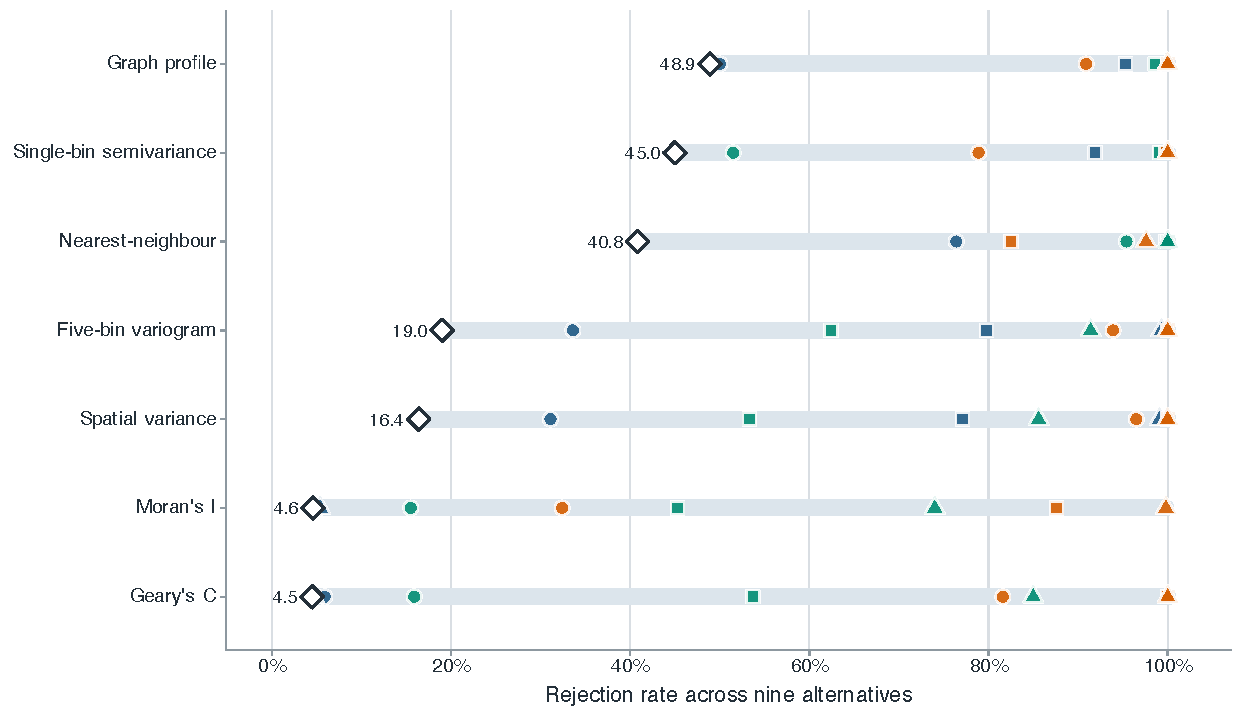
\includegraphics[width=\textwidth, height=0.62\textheight, keepaspectratio]{figure01_simulation_diagnostics.pdf}
  \caption{Power across nine simulated spatial alternatives. Blue, green and
  orange marks denote amplitude reduction, correlation-range expansion and
  gradient suppression; circles, squares and triangles denote weak, medium
  and strong changes. For each method, the pale segment spans power across the
  nine alternatives and the diamond marks the minimum.}
  \figalttext{A range-and-dot plot compares seven methods.
  Each method has nine coloured and shaped points, a pale segment spanning
  their range and a diamond at the minimum; the ranges overlap substantially.}
  \label{fig:simulation}
\end{figure}

\subsection{Calibration under temporal dependence}

The randomisation procedure remains approximately calibrated in the
simulated cyclic-invariant settings. Designs with shared structure in the
regional mean and spatial field give similar calibration, including seasonal
progression and selection of a daily regional peak. These results support
use of the complete scale profile as the randomised object under the
conditional invariance assumption. Their calibration depends on the joint structure of event labels and
dispersion profiles, beyond the mean contrast alone.

Dependence between summers primarily affects uncertainty estimation. At the
observed record length, the Student and HAC intervals under-cover when the
summer sequence is positively correlated, while the mean contrast remains
approximately centred. Preserving the actual evaluation calendar gives the
same distinction. Thus removing the development summers has little effect on
centring in these designs; estimating variation across a short dependent
record is the main difficulty. The empirical interpretation accordingly
combines the conditional randomisation result with the scale profile and the
recurrence of the contrast across summers.

\subsection{Stability of relative contrasts}

Calibration of a randomisation test can coexist with imprecise effect
estimation. In the heavy-tail designs, the raw dispersion ratio has much
greater sampling variability than its log and bounded transformations,
although their rejection behaviour is similar. The transformations reduce
the influence of extreme daily energies on the relative comparison. This
motivates reporting the raw contrast with transformation checks, so that the
scientific interpretation rests on the common spatial pattern rather than on
a single ratio scale (Supplementary Section~S10).

\section{Humid heat in eastern China}

\subsection{Study data}

We analyse synchronous ERA5-Land wet-bulb temperature fields over
105--125$^\circ$E and 20--42$^\circ$N during June--August 1991--2025
\citep{munoz2021}. The domain spans the pronounced subtropical-to-temperate
latitudinal gradient while excluding most of the Tibetan Plateau. The
primary lattice contains 121 land sites, with a nested 465-site lattice for
spatial-resolution and coverage comparisons
(Figure~\ref{fig:study-area}). The evaluation sample excludes the two
summers used for method development, as described in Section~3.

Wet-bulb temperature is derived from air temperature, dew point and surface
pressure using the thermodynamic formulation of \citet{bolton1980} and
\citet{davies2008}. Each daily field contains simultaneous values at the
hour of the maximum regional mean. This common observation time gives the
coverage measures their interpretation as concurrent spatial extent.
Within-month high and middle groups follow the definitions in Section~2.
Supplementary Section~S14 records the conversion and field-selection details.

The 1950--1990 ERA5-Land record provides a temporal extension at the same
sites. NOAA observations provide a measurement comparison on a sparse
station network, using matched event times and spatial support
\citep{smith2011}. Their distinct temporal and spatial supports are retained
in the interpretation of the results.

\begin{figure}[H]
\centering
  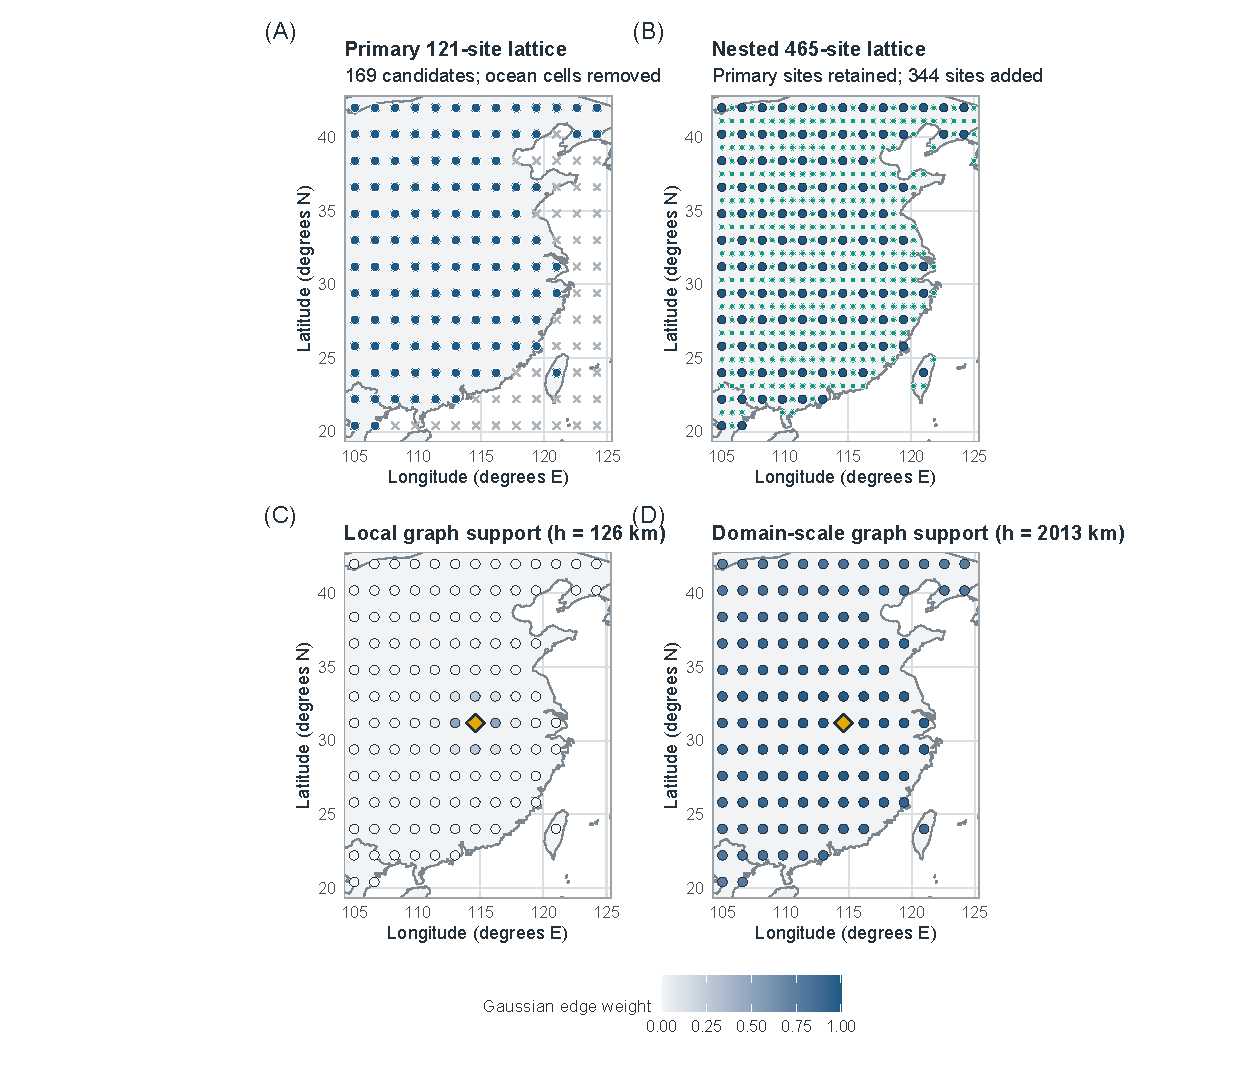
\includegraphics[width=0.90\textwidth, height=0.60\textheight, keepaspectratio]{figure02_study_area.pdf}
  \caption{Spatial sampling and graph support. (A) Analysis lattice with 121
  land sites from 169 candidates. (B) Nested lattice adding 344 land sites
  while retaining every analysis site. (C,D) Gaussian edge weights from one
  reference site under the 126- and 2,013-km graphs, showing how bandwidth
  changes the geographic support at fixed coordinates. Basemap: Natural Earth
  1:50m, accessed through the R \texttt{maps} package.}
  \figalttext{Four eastern-China maps compare the analysis and
  nested site lattices, then show weights concentrated near one reference site
  under the 126-km graph and spread across the domain under the 2,013-km graph.}
  \label{fig:study-area}
\end{figure}

\subsection{Measuring simultaneous coverage}

We measure the spatial extent of humid heat on the 465-site lattice at the
original 121-site peak time. Each retained site represents a
$0.8^\circ\times0.9^\circ$ cell clipped to the study rectangle and the
Natural Earth land polygon. WGS84 cell areas sum to 3.221 million km$^2$,
covering 95.7\% of the mapped land in that rectangle. Let $a_i$ be the
represented land area and $a_+=\sum_i a_i$. At threshold $u$, define
\begin{equation}
 A_t(u)=\frac{\sum_i a_i I(y_{it}>u)}{a_+},\qquad
 C_t(u)=\frac{\max_{B\in\mathcal B_t(u)}\sum_{i\in B}a_i}{a_+},
 \label{eq:coverage}
\end{equation}
where $\mathcal B_t(u)$ contains connected components of exceedance cells
under four-neighbour grid adjacency, with $C_t(u)=0$ when the exceedance set
is empty. Multiplication by $a_+$ gives the corresponding areas in km$^2$.
These quantities describe simultaneous coverage at the sampling resolution.
Spatial extent and contiguity are also central to temperature-event analyses
by \citet{healy2025} and \citet{skinner2025}.

The temperature range uses the 1st and 99.5th percentiles of the two
development summers, rounded outward to 0.25$^\circ$C steps. We retain all
77 thresholds from 9.5 to 28.5$^\circ$C. For each threshold we compare high
and middle days within month-year, then average months and evaluation summers
equally. The differences are expressed in area percentage points and km$^2$.
Pointwise descriptive intervals resample five-year calendar blocks of the
annual contrasts, retaining the positions of the two excluded development
years. Eight-neighbour connectivity and cosine-latitude weights provide
separate sensitivity comparisons.

We then compare how summaries of the 121-site field describe coverage on the
465-site grid. A mean-and-season regression is followed by a strong simple
baseline that also includes spatial variance, the signed latitude slope and
the area-weighted 121-site exceedance proportion. Two further models add
five binned semivariances or the five graph values, each divided by spatial
variance and log-transformed to describe relative scale structure. All four
use the same spline regression with ridge regularisation and fitted
proportions clipped to $[0,1]$. Linear spatial interpolation, followed by
coverage calculation, provides a full-field comparison.

Seven held-out five-year calendar blocks and one-year training buffers
separate evaluation from fitting. Nested blocked validation selects the
ridge penalty using training years, following the dependence-aware approach
to model assessment discussed by \citet{roberts2017}. Errors are averaged
across thresholds, then equally across months and summers, for all days and
for high days separately. An additional exceedance comparison uses only the
344 new sites. The connected-area calculation uses all 465 sites. This
comparison measures spatial information within ERA5-Land across omitted
years. Supplementary Section~S13 gives the complete definitions and fitting
procedure.


\subsection{Scale dependence of spatial contraction}

High regional wet-bulb temperature is associated with attenuation of broad
geographic contrasts. The average relative dispersion contrast is
$-7.28\%$, but the more informative feature is its increasing magnitude with
bandwidth (Figure~\ref{fig:multiscale-evidence};
Table~\ref{tab:confirm-scales}). The profile indicates that the decrease also detected by ordinary spatial
variance is concentrated in broad geographic structure, with a smaller local
component. This scale dependence provides the basis for the structural
interpretation below.

The contrast recurs across evaluation summers and is supported by the
protocol comparisons and the subsequent exploratory cyclic-shift analysis
(Supplementary Sections~S1 and S3). The latter evaluates the conditional
invariance null in Equation~\eqref{eq:cyclic-null}. The principal result
concerns differences between thermal states within summer; the estimated
change in this contrast over calendar years remains uncertain.

The earlier climate record reproduces the concentration of contraction at
broad scales (Supplementary Section~S7). Its consistency with the evaluation
period supports a recurrent spatial feature of high-mean humid heat. The
extension shares the reanalysis system, including the preliminary forcing
used for its earliest segment, so its value lies in the temporal persistence
of the scale pattern.

\begin{figure}[H]
\centering
  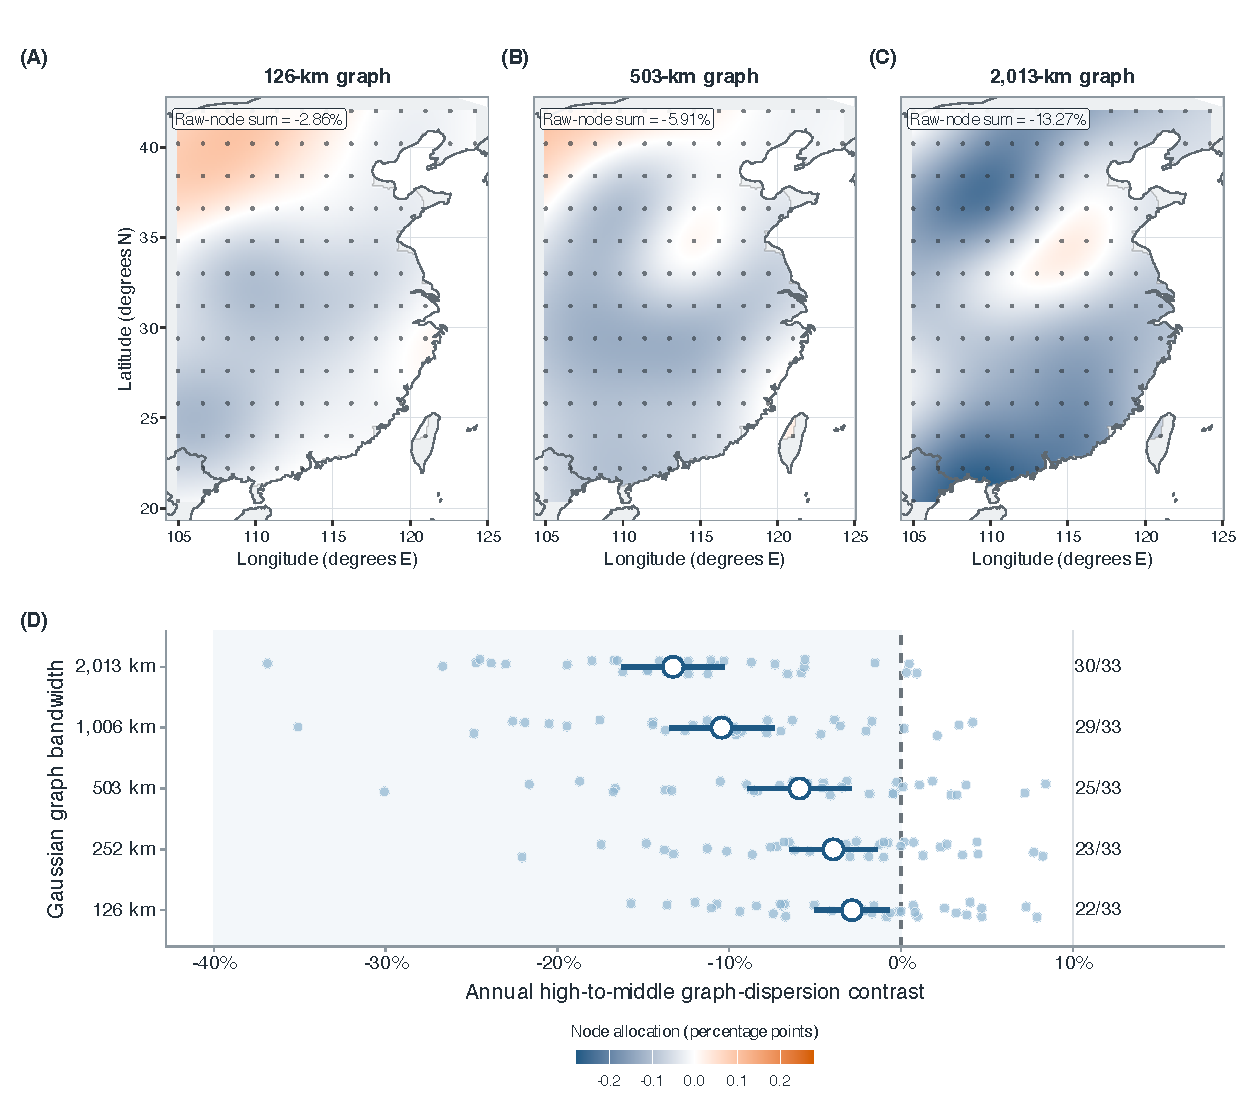
\includegraphics[width=\textwidth, height=0.62\textheight, keepaspectratio]{figure03_multiscale_evidence.pdf}
  \caption{Scale-specific node allocations and summer contrasts for the 33
  evaluation summers. (A--C) Allocations for the 126-, 503- and 2,013-km
  graphs share a symmetric colour scale; their observed-node sums are
  $-2.86\%$, $-5.91\%$ and $-13.27\%$. The interpolated surfaces visualise the
  121 observed-node values; estimation and inference use the observed nodes.
  (D) Small circles show summer-specific contrasts at all five bandwidths;
  large circles and bars show means and 95\% descriptive $(t)$-reference intervals
  based on between-summer variation. Labels
  give the numbers of negative summers.}
  \figalttext{Three smoothed eastern-China maps, each
  overlaid with the 121 analysis sites, show increasingly coherent negative
  node allocations at 126, 503 and 2,013 km. A lower panel shows the 33 annual
  contrasts at all five bandwidths, with mean contrasts and negative-summer
  counts increasing in magnitude with bandwidth.}
  \label{fig:multiscale-evidence}
\end{figure}



\subsection{Geographic extent of simultaneous humid heat}

The attenuation of broad spatial contrasts accompanies a larger connected
humid-heat footprint (Figure~\ref{fig:application-coverage}). At
24$^\circ$C, the high-minus-middle differences in total and largest connected
area are 12.91 and 12.57 percentage points, respectively, each corresponding
to approximately 400,000 km$^2$ of represented land. The coverage contrast
therefore includes substantial differences in the extent of contiguous
humid-heat regions.

Threshold dependence is central to this interpretation. The area separation
is greatest around 23--24$^\circ$C and narrows towards the highest thresholds.
The geographic expression of high regional humid heat consequently depends
on the temperature level being considered. Spatial contraction alone does
not determine this curve: regional mean and spatial pattern change together
between the groups. Direct coverage measurement establishes the extent of
their combined association.

\begin{figure}[H]
\centering
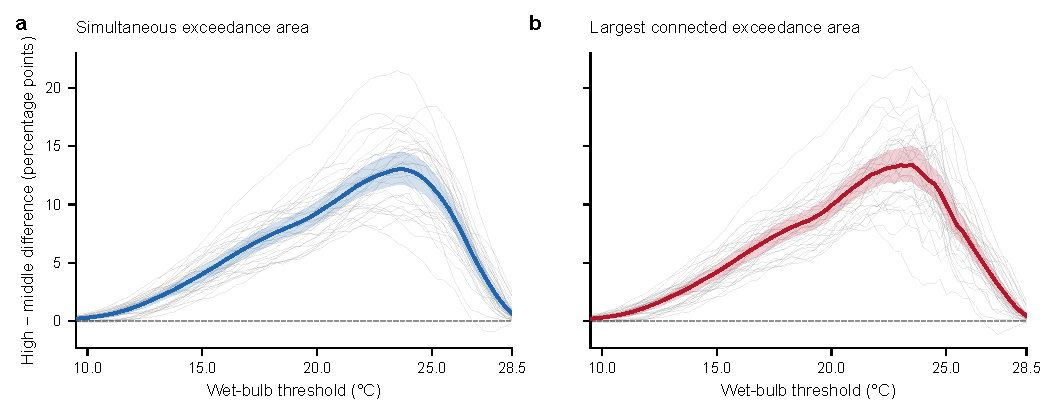
\includegraphics[width=\textwidth]{application_coverage.pdf}
\caption{High-minus-middle differences in simultaneous humid-heat coverage
at the original daily peak times. (a) Total exceedance area. (b) Largest
four-neighbour connected exceedance area. Thick curves average months and
33 evaluation summers equally; thin grey curves show every summer. Shading
gives pointwise 95\% percentile intervals from 1,999 resamples of five-year
calendar blocks. All 77 development-defined temperature thresholds are shown.
Areas refer to the 3.221-million-km$^2$ represented land support.}
\figalttext{Both area-difference curves rise from small positive values at low
thresholds to approximately thirteen percentage points near 24 degrees
Celsius, then decline toward the upper end of the threshold range. Grey
annual curves show variation between summers, including some negative values
at high thresholds.}
\label{fig:application-coverage}
\end{figure}

The comparison of spatial summaries identifies where most coverage
information resides (Table~\ref{tab:application-comparison}). The principal
reduction in error occurs when the regional mean is supplemented by simple
spatial summaries. Distance-resolved predictors provide small further
improvements, with graph and variogram representations performing similarly.
The same conclusion holds for the additional-site reference. Thus coverage
estimation and structural interpretation have different informational
requirements: the simple summaries describe geographic extent well, while
the graph profile connects regional dispersion to its spatial scales and
components. The magnitude and annual consistency of the incremental gains
are documented in Supplementary Section~S13.

\begin{table}[!t]
\centering\small
\caption{Held-out mean absolute error in area percentage points. Errors are
averaged over all 77 thresholds (9.5--28.5$^\circ$C at 0.25$^\circ$C steps),
then equally over months and 33 evaluation summers. All-day errors use 3,036
June--August daily fields in 1991--2025 excluding 2015 and 2022; high-day errors
use the 792 original upper-quartile days. The last two columns use the 344
additional sites. All inputs come from the original 121 sites.}
\label{tab:application-comparison}
\begin{tabular}{@{}lrrrrrr@{}}
\toprule
& \multicolumn{2}{c}{Exceedance area} & \multicolumn{2}{c}{Largest component} & \multicolumn{2}{c}{Additional sites}\\
\cmidrule(lr){2-3}\cmidrule(lr){4-5}\cmidrule(lr){6-7}
Method & All & High & All & High & All & High\\
\midrule
Mean and season & 2.794 & 2.291 & 3.070 & 2.593 & 2.818 & 2.314 \\
Strong simple baseline & 0.827 & 0.747 & 1.389 & 1.268 & 1.028 & 0.929 \\
Simple + variogram & 0.815 & 0.741 & 1.366 & 1.266 & 1.013 & 0.922 \\
Simple + graph & 0.820 & 0.743 & 1.379 & 1.265 & 1.020 & 0.925 \\
Spatial interpolation & 1.398 & 1.414 & 1.823 & 1.859 & 1.861 & 1.882 \\
\bottomrule
\end{tabular}
\end{table}



\subsection{Latitudinal structure of the contraction}

The broad-scale association is concentrated in the persistent latitudinal
gradient. Relative to each day's regional mean, high-day fields are warmer
in the north and cooler in the south than middle-day fields
(Figure~\ref{fig:spatial-decomposition}). The spatial allocations therefore
identify attenuation of a familiar climatic contrast as the main geographic
expression of the regional statistic.

\begin{figure}[H]
\centering
  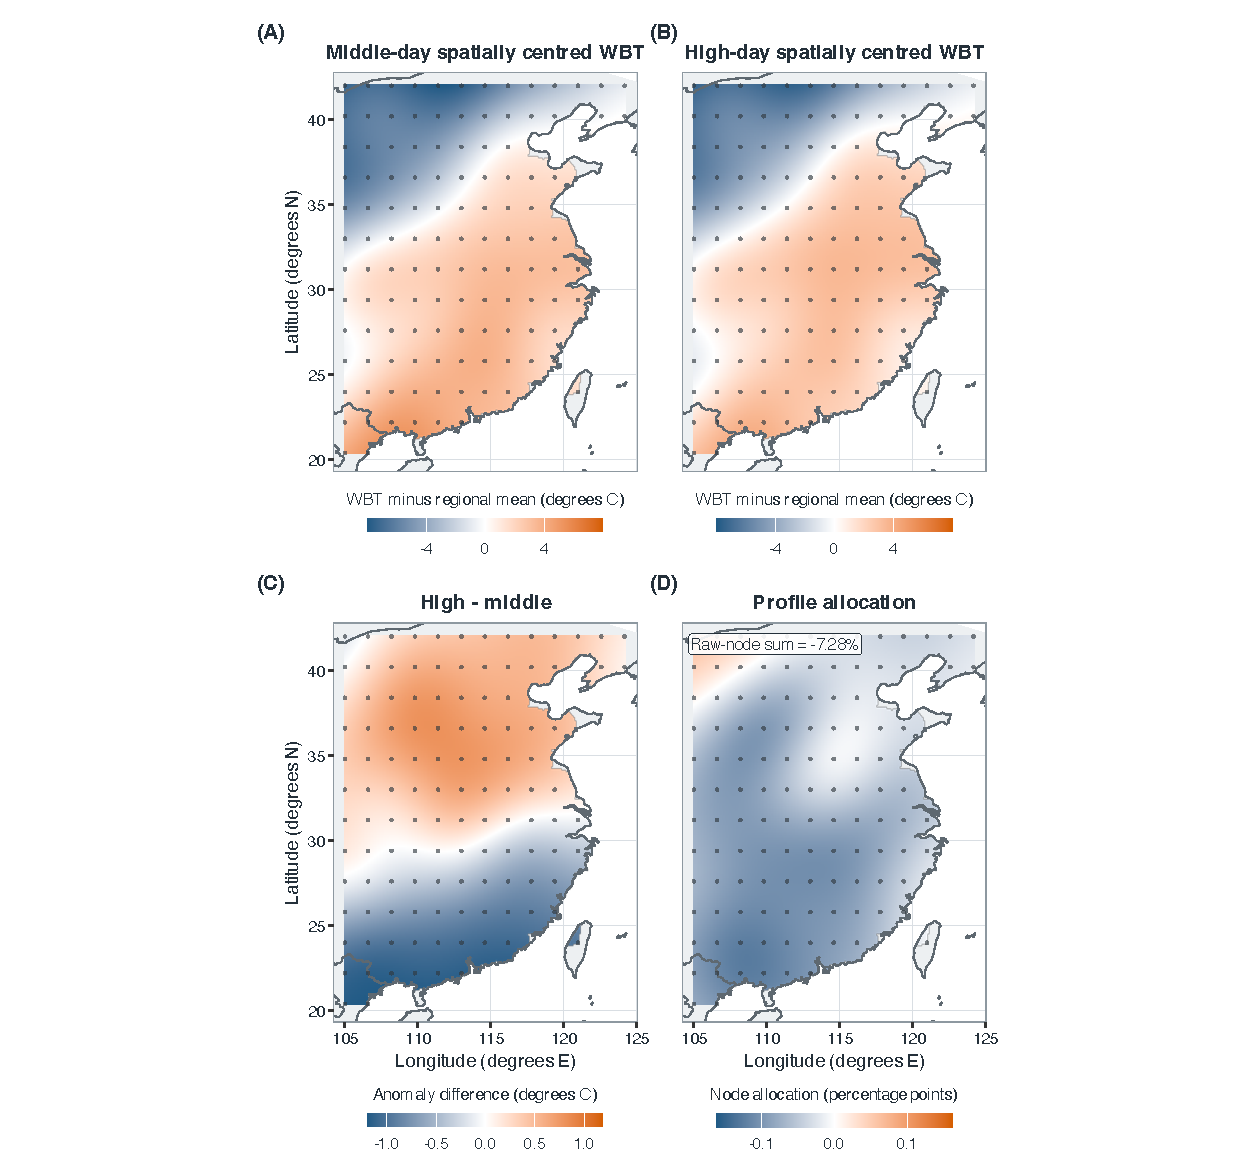
\includegraphics[width=0.90\textwidth, height=0.60\textheight, keepaspectratio]{figure04_primary_spatial_decomposition.pdf}
  \caption{Spatial structure of the 121-site evaluation contrast.
  (A,B) Middle- and high-day spatially centred fields; (C) their difference;
  (D) exact observed-node allocations averaged over the five
  graph scales. The 121 allocations sum to $-7.28\%$, identical to the
  five-scale estimand. The interpolated surfaces visualise the 121
  observed-node values; estimation and inference use the observed nodes.}
  \figalttext{Four smoothed eastern-China maps derived from
  121 analysis sites, shown as dots. The spatially centred surfaces show a weaker
  north--south contrast on high days; the
  high-minus-middle surface changes from positive in the north to negative in
  the south, and most observed-node allocations are negative, with the
  strongest negative values concentrated in the central and southern parts
  of the domain.}
  \label{fig:spatial-decomposition}
\end{figure}

The climatology decomposition gives this pattern a more specific
interpretation. High-day anomalies oppose the monthly climatological
pattern more strongly, while their own broad-scale energy changes little
(Figure~\ref{fig:energy-decomposition}). The decline in total dispersion
appears primarily in the signed alignment between these two fields.
Regional coherence can therefore increase through compensation of a
persistent gradient, with comparatively little change in the magnitude of
transient spatial anomalies.

The projection analyses support this interpretation. Latitude accounts for
most of the resolved broad geographic component; including longitude and
elevation preserves the conclusion about the total structured component.
Re-estimating climatology without the evaluated summer has little effect on
the decomposition. Together, these checks associate the contraction with the
observed climatic gradient rather than a particular fitted reference field
(Supplementary Section~S5).

\begin{figure}[H]
\centering
  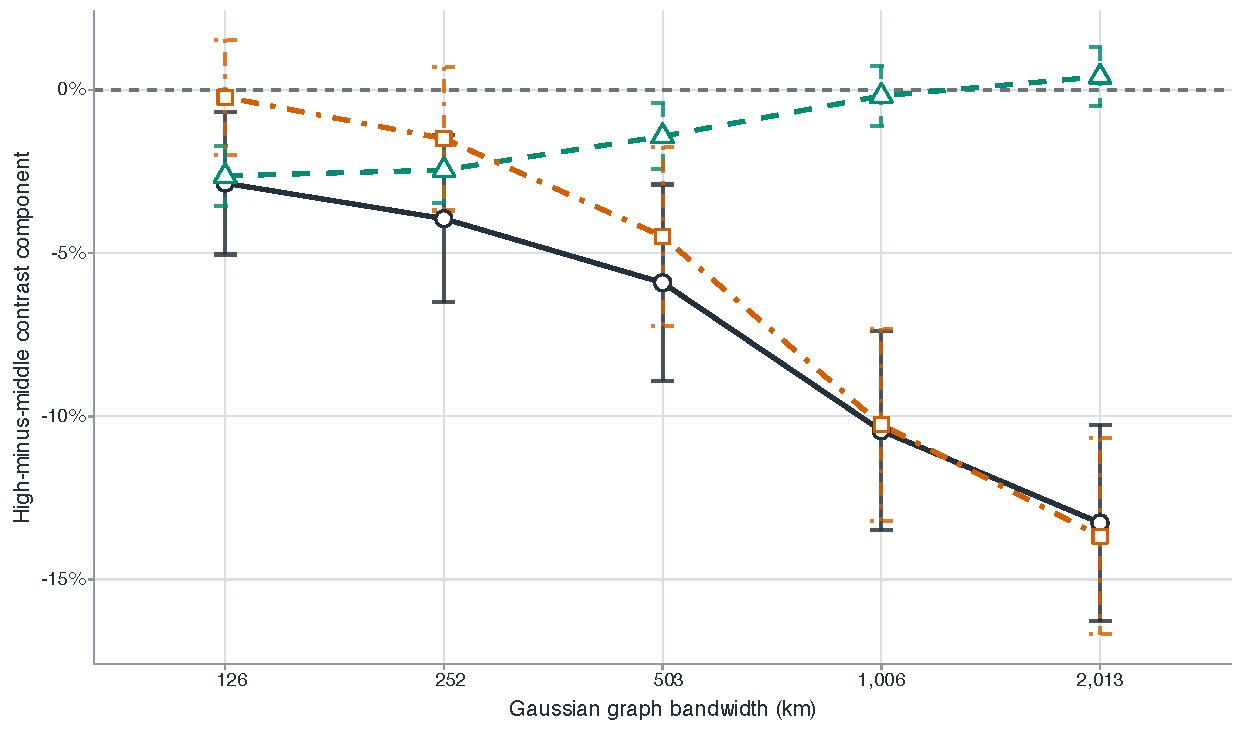
\includegraphics[width=0.92\textwidth, height=0.60\textheight, keepaspectratio]{figure05_energy_decomposition.pdf}
  \caption{Exact decomposition of the raw-field graph contrast. Dark circles,
  teal triangles and orange squares denote total change, anomaly-energy change
  and the climatology--anomaly cross component; bars are 95\% descriptive
  intervals. Monthly-climatology energy cancels within each record.}
  \figalttext{Across five bandwidths, dark circles become
  increasingly negative. Teal triangles remain near zero at broad scales,
  while orange squares closely follow the negative total.}
  \label{fig:energy-decomposition}
\end{figure}

\begin{table}[H]
\centering
\caption{Physical scale of the evaluation-period graph contrasts. $h$ is the
Gaussian bandwidth. $\bar d_w$ is the
edge-weighted mean pair distance, and $N_{\mathrm{eff}}$ is the Kish effective
edge count. Graph contrasts are relative changes in weighted squared
differences. RMS contrasts average record-specific ratios of
$(2Q)^{1/2}$; Negative is the number of negative summer graph contrasts.}
\label{tab:confirm-scales}
\small
\setlength{\tabcolsep}{4.5pt}
\begin{tabular}{rrrrrr}
\toprule
$h$ & $\bar d_w$ & $N_{\mathrm{eff}}$ & Graph contrast & RMS contrast & Negative \\
(km) & (km) & (edges) & (\%) & (\%) & (/33) \\
\midrule
126   & 200 & 366   & $-2.86$  & $-1.54$ & 22 \\
252   & 319 & 1,138 & $-3.94$  & $-2.14$ & 23 \\
503   & 549 & 3,223 & $-5.91$  & $-3.25$ & 25 \\
1,006 & 826 & 6,005 & $-10.44$ & $-5.70$ & 29 \\
2,013 & 992 & 7,109 & $-13.27$ & $-7.22$ & 30 \\
\bottomrule
\end{tabular}
\end{table}

\subsection{Sensitivity of the structural interpretation}

Graph weighting, distance definitions and sampling density change the
estimated magnitude while preserving the broad scale ordering. Domain
changes are more consequential because they alter the geographic gradient
represented by the field. The contrast is thus a property of the specified
spatial support, and its scale profile is more stable across these choices
than any single regional percentage (Figure~\ref{fig:application-robustness};
Supplementary Section~S6).

Field definition has a clearer substantive effect. Removing site climatology
substantially attenuates the contrast, consistent with the structural
decomposition. Fixed-hour and daily-mean fields retain the negative
association, and the continuous-intensity analysis extends it beyond the
quartile grouping. Calendar matching gives a weaker contrast on its
restricted set of eligible day pairs while preserving scale ordering.
These comparisons distinguish variation in the climatic field from
sensitivity to how days are selected; the underlying definitions and results
are given in Supplementary Sections~S9, S12 and S14.

\begin{figure}[H]
\centering
  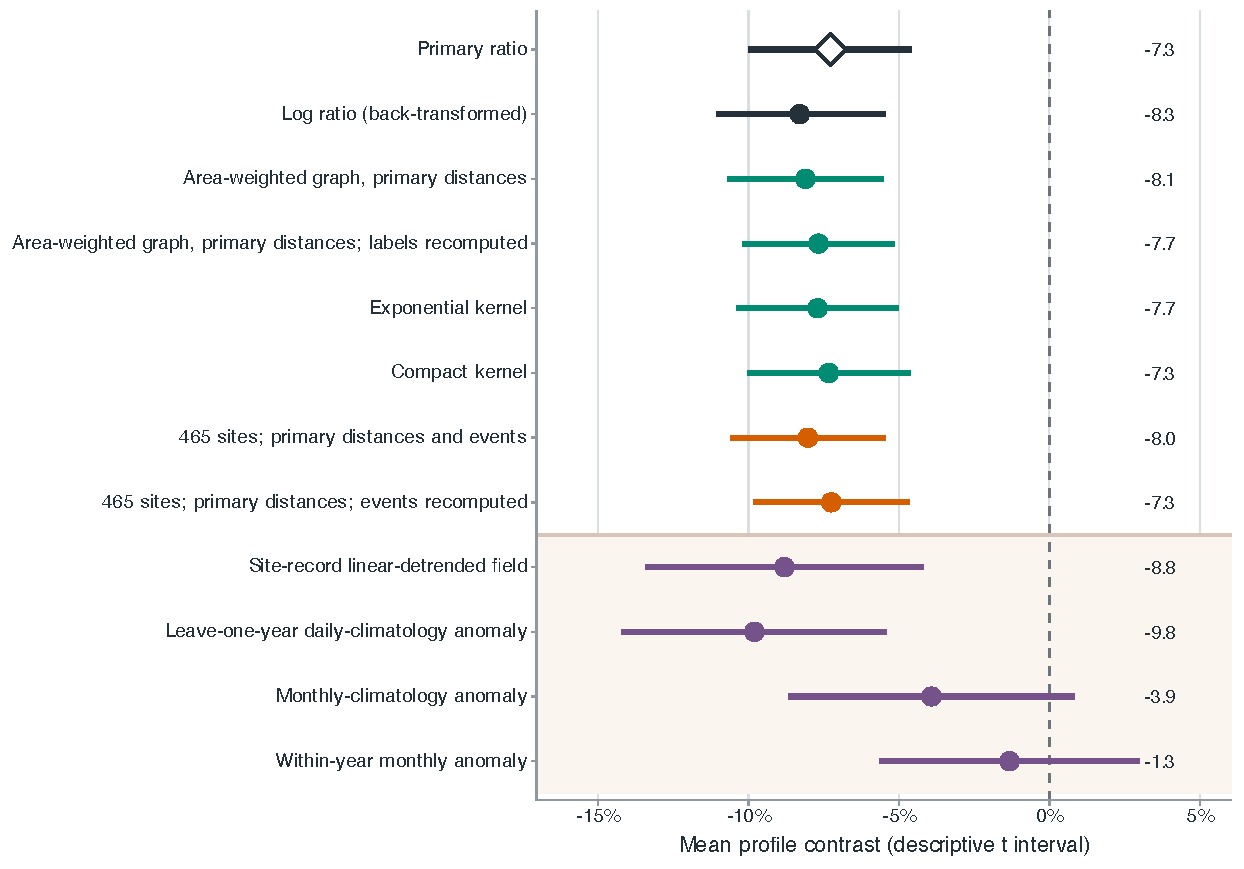
\includegraphics[width=\textwidth, height=0.62\textheight, keepaspectratio]{figure06_application_robustness.pdf}
  \caption{Robustness of the mean profile contrast. Dark rows denote the main
  and transformation analyses; green, orange and purple rows denote graph
  construction, spatial resolution and field definition. Points and bars are
  estimates and descriptive $t$-reference intervals based on between-summer
  variation.}
  \figalttext{A forest plot shows mostly overlapping negative
  estimates across transformation, graph and resolution choices. Two
  purple-shaded anomaly-field rows lie closest to zero.}
  \label{fig:application-robustness}
\end{figure}

The station comparison supports the broad geographic interpretation
(Figure~\ref{fig:noaa-validation}). Reanalysis and station observations show
concordant contraction at the scales supported by the station network,
whereas local contrasts are less precisely determined. The broad direction
also persists with station-defined events and fixed spatial support.
Stricter availability requirements widen uncertainty by reducing the retained
record. The comparison therefore provides complementary measurement evidence
for the broad pattern at common events, with the greatest uncertainty at
short distances (Supplementary Section~S8).

\begin{figure}[H]
\centering
  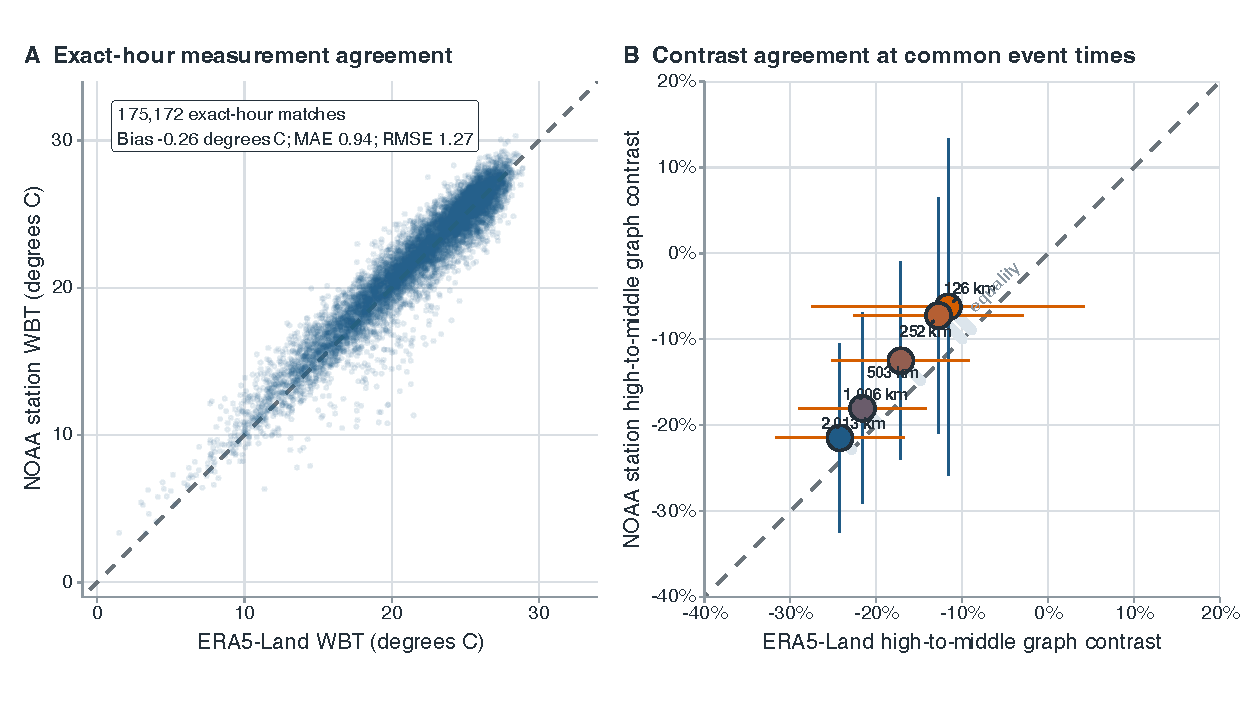
\includegraphics[width=\textwidth, height=0.62\textheight, keepaspectratio]{figure07_noaa_agreement.pdf}
  \caption{NOAA station and ERA5-Land agreement in ten station-comparison
  summers. (A) Exact-hour WBT at 28 stations, with summaries from
  all 175,172 matches. (B) High--middle graph contrasts at the five
  bandwidths, using ERA5-Land peak times and labels and identical station
  subsets. Dashed diagonals denote equality. Horizontal and vertical bars in
  panel B are paired descriptive $t$-reference intervals based on
  between-summer variation.}
  \figalttext{Two panels compare NOAA stations with
  ERA5-Land. Exact-hour WBT points in the left panel cluster around the
  equality line. In the right panel, station and ERA5-Land high--middle
  contrasts are negative at all five bandwidths and become more negative as
  the bandwidth increases; station estimates are slightly closer to zero.}
  \label{fig:noaa-validation}
\end{figure}

\section{Discussion}

The dominant spatial change on high regional wet-bulb temperature days is an
attenuation of broad climatic differences. At these scales, the daily anomaly field retains
comparable energy, but its alignment with the monthly climatology shifts
towards compensation of the latitudinal gradient. This distinction gives
a climatic interpretation to the dispersion result:
a smaller regional variance can reflect weaker persistent geographic
contrasts even when transient spatial variability remains substantial.

The coverage analysis establishes the geographic extent associated with
these thermal states. High-mean days have more extensive simultaneous
exceedance and larger connected humid-heat regions, with the greatest area
separation in an intermediate part of the temperature range. Regional mean,
spatial dispersion and exceedance area describe different aspects of this
state. Their joint interpretation distinguishes a broad humid-heat footprint
from the scale and structure of variation within it. The observed coverage
difference combines changes in regional level and spatial pattern.

The statistical contribution is an additive formulation that connects the
regional contrast to its scale profile and spatial components. Site
allocations and projections recover the same relative quantity used in the
regional comparison, allowing the climatic gradient to be examined within
that common measure. The application shows the interpretive value of this
connection. Simple spatial summaries already retain most information about
coverage, while the graph decomposition identifies where in scale and
geographic structure the dispersion change occurs. Structural interpretation
and coverage estimation are therefore distinct uses of the spatial data.

The evidence is strongest for broad spatial structure on the analysed
support. Sampling resolution limits local interpretation, and dependence
between summers affects the precision of inference from the available
record. Long-term changes in China's latitudinal wet-bulb temperature
pattern have been associated with heterogeneous water-vapour changes
\citep{wang2024}. Our event-scale comparison identifies a recurrent spatial configuration of
high humid heat: weaker broad climatic contrasts together with a more
extensive connected footprint.

\section*{Data availability}

ERA5-Land is available from the Copernicus Climate Data Store
(\url{https://cds.climate.copernicus.eu/datasets/reanalysis-era5-land}). The
NOAA ISD station archive \citep{smith2011} is available at
\url{https://www.ncei.noaa.gov/products/land-based-station/integrated-surface-database}.
Code and retained results for this version are archived at
\url{https://github.com/Stork343/eastern-china-wet-bulb-contraction/releases/tag/jrssc-submission-v8-2026-09-08}.
The accompanying \texttt{jrssc\_reproducibility\_bundle.zip} contains the
current manuscript, analysis code, protocols, site and station manifests,
and retained results, including the September coverage comparison.
Its \texttt{code/revision\_202609/README.md} gives the application-analysis
entry points; \texttt{output\_revision\_application/} contains the fixed
specification, coverage curves, held-out predictions and annual comparisons.
Provider-data download and field-construction programs are included. The raw
reanalysis and station archives are obtained from the providers above.

\section*{Acknowledgements}

OpenAI Codex was used for language editing, code development and checking,
and assistance with data analysis. The authors
reviewed all changes and take full responsibility for the manuscript and
analysis.

\section*{Funding}

This work was supported by the Beijing Natural Science Foundation, ``Theory,
Methodology and Applications of Functional Hierarchical Quantile Regression
Modeling'' (grant 1242005); the Fundamental Research Funds for the Central
Universities and the Research Funds of Renmin University of China, ``Robust
Statistical Inference for Complex Data'' (grant 25XNN015); and the Ministry of
Education Humanities and Social Sciences Research General Project, ``Research
on Spatial-temporal Quantile Regression Modeling: Theoretical Methods and
Applications'' (grant 25YJA910005).

\section*{Conflict of interest}

The authors declare no conflict of interest.

\small
\begin{thebibliography}{99}

\bibitem[Andrews(1991)]{andrews1991}
Andrews, D.W.K. (1991). Heteroskedasticity and autocorrelation consistent
covariance matrix estimation. \textit{Econometrica}, 59, 817--858.

\bibitem[Bolton(1980)]{bolton1980}
Bolton, D. (1980). The computation of equivalent potential temperature.
\textit{Monthly Weather Review}, 108, 1046--1053.

\bibitem[Chagnaud et~al.(2025)]{chagnaud2025}
Chagnaud, G., Taylor, C.M., Jackson, L.S., Birch, C.E., Marsham, J.H. and
Klein, C. (2025). Wet-bulb temperature extremes locally amplified by wet
soils. \textit{Geophysical Research Letters}, 52, e2024GL112467.

\bibitem[Cressie(1993)]{cressie1993}
Cressie, N.A.C. (1993). \textit{Statistics for Spatial Data}, revised edn.
New York: Wiley.

\bibitem[Davies-Jones(2008)]{davies2008}
Davies-Jones, R. (2008). An efficient and accurate method for computing the
wet-bulb temperature along pseudoadiabats. \textit{Monthly Weather Review},
136, 2764--2785.

\bibitem[Dong et~al.(2016)]{dong2016}
Dong, X., Thanou, D., Frossard, P. and Vandergheynst, P. (2016). Learning
Laplacian matrix in smooth graph signal representations.
\textit{IEEE Transactions on Signal Processing}, 64, 6160--6173.

\bibitem[Garc\'ia-Soid\'an et~al.(2004)]{garciasoidan2004}
Garc\'ia-Soid\'an, P.H., Febrero-Bande, M. and Gonz\'alez-Manteiga, W.
(2004). Nonparametric kernel estimation of an isotropic variogram.
\textit{Journal of Statistical Planning and Inference}, 121, 65--92.
doi:10.1016/S0378-3758(02)00507-4.

\bibitem[Geary(1954)]{geary1954}
Geary, R.C. (1954). The contiguity ratio and statistical mapping.
\textit{The Incorporated Statistician}, 5, 115--145.

\bibitem[Harris(2020)]{harris2020}
Harris, K.D. (2020). A shift test for independence in generic time series.
\textit{arXiv:2012.06862}.

\bibitem[Healy et~al.(2025)]{healy2025}
Healy, D., Tawn, J., Thorne, P. and Parnell, A. (2025). Inference for extreme
spatial temperature events in a changing climate with application to Ireland.
\textit{Journal of the Royal Statistical Society: Series C}, 74, 275--299.
doi:10.1093/jrsssc/qlae047.

\bibitem[Horton et~al.(2015)]{horton2015}
Horton, D.E., Johnson, N.C., Singh, D., Swain, D.L., Rajaratnam, B. and
Diffenbaugh, N.S. (2015). Contribution of changes in atmospheric circulation
patterns to extreme temperature trends. \textit{Nature}, 522, 465--469.

\bibitem[Ibragimov and Linnik(1971)]{ibragimov1971}
Ibragimov, I.A. and Linnik, Y.V. (1971). \textit{Independent and Stationary
Sequences of Random Variables}. Groningen: Wolters-Noordhoff.

\bibitem[Moran(1950)]{moran1950}
Moran, P.A.P. (1950). Notes on continuous stochastic phenomena.
\textit{Biometrika}, 37, 17--23.

\bibitem[Mu\~noz-Sabater et~al.(2021)]{munoz2021}
Mu\~noz-Sabater, J. et al. (2021). ERA5-Land: a state-of-the-art global
reanalysis dataset for land applications. \textit{Earth System Science Data},
13, 4349--4383.

\bibitem[Newey and West(1987)]{newey1987}
Newey, W.K. and West, K.D. (1987). A simple, positive semi-definite,
heteroskedasticity and autocorrelation consistent covariance matrix.
\textit{Econometrica}, 55, 703--708.

\bibitem[Pepin et~al.(2015)]{pepin2015}
Pepin, N.C. et al. (2015). Elevation-dependent warming in mountain regions
of the world. \textit{Nature Climate Change}, 5, 424--430.

\bibitem[Phipson and Smyth(2010)]{phipson2010}
Phipson, B. and Smyth, G.K. (2010). Permutation $p$-values should never be
zero: calculating exact $p$-values when permutations are randomly drawn.
\textit{Statistical Applications in Genetics and Molecular Biology}, 9,
Article 39.

\bibitem[Raymond et~al.(2020)]{raymond2020}
Raymond, C., Matthews, T. and Horton, R.M. (2020). The emergence of heat and
humidity too severe for human tolerance. \textit{Science Advances}, 6,
eaaw1838.

\bibitem[Roberts et~al.(2017)]{roberts2017}
Roberts, D.R. et al. (2017). Cross-validation strategies for data with temporal,
spatial, hierarchical, or phylogenetic structure. \textit{Ecography}, 40,
913--929. doi:10.1111/ecog.02881.

\bibitem[Seneviratne et~al.(2010)]{seneviratne2010}
Seneviratne, S.I., Corti, T., Davin, E.L., Hirschi, M., Jaeger, E.B.,
Lehner, I., Orlowsky, B. and Teuling, A.J. (2010). Investigating soil
moisture--climate interactions in a changing climate: a review.
\textit{Earth-Science Reviews}, 99, 125--161.

\bibitem[Sherwood and Huber(2010)]{sherwood2010}
Sherwood, S.C. and Huber, M. (2010). An adaptability limit to climate change
due to heat stress. \textit{Proceedings of the National Academy of Sciences},
107, 9552--9555.

\bibitem[Shreevastava et~al.(2023)]{shreevastava2023}
Shreevastava, A., Raymond, C. and Hulley, G. (2023). Contrasting intraurban
signatures of humid and dry heatwaves over Southern California.
\textit{Journal of Applied Meteorology and Climatology}, 62, 709--720.

\bibitem[Shuman et~al.(2013)]{shuman2013}
Shuman, D.I., Narang, S.K., Frossard, P., Ortega, A. and Vandergheynst, P.
(2013). The emerging field of signal processing on graphs: extending
high-dimensional data analysis to networks and other irregular domains.
\textit{IEEE Signal Processing Magazine}, 30, 83--98.

\bibitem[Simmons et~al.(2011)]{simmons2011}
Simmons, J.P., Nelson, L.D. and Simonsohn, U. (2011). False-positive
psychology: undisclosed flexibility in data collection and analysis allows
presenting anything as significant. \textit{Psychological Science}, 22,
1359--1366.

\bibitem[Skinner et~al.(2025)]{skinner2025}
Skinner, C.B., Touma, D., Barlow, M., Singh, D. and King, T. (2025).
The spatial extent of heat waves has changed over the past four decades.
\textit{Communications Earth \& Environment}, 6, 662.
doi:10.1038/s43247-025-02661-y.

\bibitem[Smith et~al.(2011)]{smith2011}
Smith, A., Lott, N. and Vose, R. (2011). The integrated surface database:
recent developments and partnerships. \textit{Bulletin of the American
Meteorological Society}, 92, 704--708. doi:10.1175/2011BAMS3015.1.

\bibitem[Speizer et~al.(2022)]{speizer2022}
Speizer, S., Raymond, C., Ivanovich, C. and Horton, R.M. (2022). Concentrated
and intensifying humid heat extremes in the IPCC AR6 regions.
\textit{Geophysical Research Letters}, 49, e2021GL097261.

\bibitem[Stull(2011)]{stull2011}
Stull, R. (2011). Wet-bulb temperature from relative humidity and air
temperature. \textit{Journal of Applied Meteorology and Climatology}, 50,
2267--2269.

\bibitem[Wang et~al.(2024)]{wang2024}
Wang, F., Gao, M., Liu, C., Zhao, R. and McElroy, M.B. (2024).
Uniformly elevated future heat stress in China driven by spatially
heterogeneous water vapor changes. \textit{Nature Communications}, 15, 4522.
doi:10.1038/s41467-024-48895-w.


\bibitem[White(2000)]{white2000}
White, H. (2000). A reality check for data snooping. \textit{Econometrica},
68, 1097--1126.

\bibitem[Wood(2003)]{wood2003}
Wood, S.N. (2003). Thin plate regression splines. \textit{Journal of the Royal
Statistical Society: Series B}, 65, 95--114.

\bibitem[Yuan and Shou(2024)]{yuan2024}
Yuan, A.E. and Shou, W. (2024). A rigorous and versatile statistical test for
correlations between stationary time series. \textit{PLOS Biology}, 22,
e3002758.


\end{thebibliography}

\end{document}
